\cleardoublepage

\addcontentsline{toc}{chapter}{\numberline{} Le problème de l’arbre dominant DTP }
\addtocontents{lof}{\textbf{ Le problème de l’arbre dominant DTP }}

\setcounter{chapter}{3}
\setcounter{section}{0}
\setcounter{figure}{0}

\begin{center}
	\Huge\textbf{ Le problème de l’arbre dominant DTP }
\end{center}

\section{Introduction}
Comme la gestion de l’énergie dans les réseaux de capteurs sans fil (RCSFs) est très exigeante, plusieurs chercheurs sont actuellement engagés non seulement dans le développement des technologies requises au niveau des différentes couches de la pile protocolaire des réseaux de capteurs, mais aussi pour la conception des méthodes et des algorithmes qui assurent une gestion meilleure.

Au cours de ces dernières années, les chercheurs sont arrivés à représenter un réseau sous forme d’un graphe G, où chaque capteur sera représenté par un nœud et la connexion entre deux nœuds est représentée par une arête. Néanmoins, cela ne résout pas  les problèmes de routage pour la gestion d’énergie dans les RCSFs, alors ils ont pensé à la notion du plus court chemin dans G.  Cette approche a donné naissance à un nouveau problème nommé le problème de ensemble dominant (Connected Dominating Set CDS).

Cette approche a été largement utilisée pour construire une ossature de routage dans les réseaux de capteurs \cite{thai2008construction,thai2007connected}. Elle se concentre sur les nœuds au lieu des arêtes afin de minimiser la consommation d’énergie. Tandis que l’énergie dissipée lors du routage des données est directement liée aux arêtes.
Le problème de l’arbre dominant (Dominating Tree Problem ou DTP) a donc été formulé dans le but de pallier aux lacunes du CDS \cite{shin2010approximation,zhang2008new} .

Dans ce chapitre, nous présenterons le problème de l’arbre dominant, puis nous synthétiserons quelques travaux effectués pour sa résolution, enfin nous clôturerons ceci par une conclusion.


\section{Définition du problème}
Le problème de l’arbre dominante nous incite à trouver un arbre de poids minimal DT. Le principe est que chaque réseau sans fil sera représenté par un graphe pondéré non orienté G=(V,E,w), où V est l’ensemble des nœuds du réseau, E l’ensemble des liaisons de communication du réseau et w un poids non négatif attribué pour chaque arête e=(u,v). Chaque nœud $v \in V$, est soit dans DT, soit adjacent à un nœud déjà dans DT. La complexité de la construction d’un arbre dominant est Np-hard.
 
D’autre part, la résolution du DTP peut générer une ossature de routage pour les protocoles de diffusion puisque chaque nœud n’a pas à construire son propre arbre de diffusion, alors ils utilisent l'ossature virtuelle pour réduire la surcharge de message et le poids de l'ossature qui représente la consommation d'énergie minimisée. Comment régler le problème de l’arbre dominant (DTP)? 


\section{Complexité et approximation}
Le problème de l’arbre dominant (DTP) est une variante récente d’ensemble dominants en théorie des graphes. Il est prouvé qu'il est un problème N P-Hard \cite{shin2010approximation,zhang2008new}.

L’arbre de Steiner est souvent associé à des problème de conception de réseau. Le principe de conception de cet arbre est très proche du principe de conception de l’arbre dominant. Il consiste à construire un arbre de poids minimal r nommé DST, en veillant à ce qu'il y ait au moins un chemin allant de la racine à chaque nœud de l'ensemble D tel que D est un ensemble dominant minimal appartenant à V dans G.

Dans \cite{shin2010approximation} il a été montré que le DTP peut être réduit au problème DST en un temps polynomial. Rappelons que l’algorithme de construction de DST avec la conservation du rapport de performance nous permet de l’ appliquer au DTP de la façons suivante:\\
Dans le problème DT nous introduisons un sommet factrice v* ( un faux sommet) pour chaque sommet réel $v \in V$,  puis nous ajoutons les arcs pour tous les voisins de v (y compris v lui-même) au nœud factice v, et fixons le poids à zéro pour toute arrête nouvellement ajoutées. De même, pour les arêtes originales, l’arête est bidirectionnelle et le poids identique à celui du graphe original. Dans le nouveau graphe orienté G’ = (V’, E’, w’), si nous choisissons un $v’ \in V’$ arbitraire comme root r, et que tous les sommets factices soient des terminaux, nous pouvons obtenir un DST basé sur un algorithme DST existant \cite{zhang2008new} et obtenir ainsi un DT de G. Il est clair que la réduction est réalisée en temps linéaire. Cette réduction est illustrée sur la Figure \ref{fig:31}.

\begin{figure}[H]
	\centering
	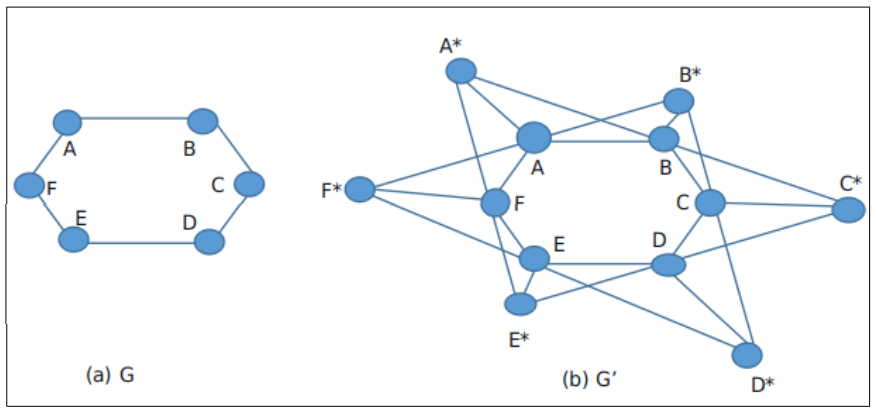
\includegraphics[width=15cm,height=6cm]{Chap3/1.png}
	\caption{Exemple de réduction du graphe G en G’}
	\label{fig:31}
\end{figure}

\textbf{Lemme 1:}
Si r est dans le DT optimal, alors le DT introduit par DST aura le même poids optimal. En outre, l’utilisation de l’algorithme d’approximation pour le problème DST aura le même rapport d’approximation pour le problème DT \cite{shin2010approximation}.

\textbf{Preuve:}
Supposons qu'il existe une arborescence dominante optimale DT*, nous pouvons faire en sorte que tous les nœuds de DT* apparaissent dans le DST. Puisque r est dans DT*, pour chaque nœud de DT, au moins un de ses voisins doit être dans DT, et pour tout terminal, nous pouvons ajouter un front dirigé depuis ce voisin. Et nous savons que ces arêtes sont pondérées à zéro, de sorte que le poids de cette DST est égal à w (DT*). Supposons qu'il existe un DST optimal ST*, alors nous avons w (DT*) $\geq w$ (ST*). En outre, pour un DST optimal, nous pouvons éliminer toutes ces arêtes pondérées par zéro. Étant donné que tous les nœuds terminaux ont un chemin allant de r à eux, chaque nœud aura au moins un de ses voisins figurant dans cet arbre, ce qui signifie qu’il s’agit d’un DT. Nous avons donc w (ST*) $ \geq w$ (DT*). En conclusion, nous avons w (DT*) = w (ST*). Cela implique à son tour que nous pouvons obtenir le même rapport de performances pour le problème DT que pour le DST \cite{shin2010approximation}.

Une approximation poly-logarithmique a été fourni par les auteurs dans \cite{charikar1999approximation}.  L’algorithme qui  nous permet d’obtenir le rapport de performance est le suivant :

\begin{algorithm}[H]
\label{alg3:RSDT}
\caption{Recuit simulé}
\KwData{un graphe général pondéré non orienté $G=(V, E, w)$}
\KwResult{Un DT de $G$ }
\SetAlgoLined
\DontPrintSemicolon

Initialiser une liste pour sauvegarder le DT et son poids \;
Trouver un sommet factice u en G avec un degré minimum \;
Transformer $G$ en $G’ = (V’, E’, w’)$ en utilisant la technique de transformation\;
\For{chaque nœud $v$ où $(u, v) \in E $}{
	Exécution de l'algorithme DST \cite{charikar1999approximation} dans G et définir v comme racine r pour obtenir un DT \;
	Sauvegarder le DT et son poids dans la liste \;	
}
 Retourner le DT avec poids minimum dans la liste \;
\end{algorithm}


L’algorithme \ref{alg3:RSDT} nous permet de transformer le DTP en DST. Puis nous pouvons appliquer l’algorithme dans \cite{charikar1999approximation} qui va nous permettre par la suite de résoudre le problème DST et de trouver une solution pour le DTP. Cela n’est possible que si le sommet racine r choisie dans l’algorithme \ref{alg3:RSDT} soit le meilleur choix ( r doit être dans le DT optimal). Au final, nous pouvons revenir à l’état initial de  notre graphe de départ en supprimant les nœuds factrices ajoutés ainsi que leurs arêtes. 


\section{Notions de base}

\subsection{Arbre couvrant de poids minimal (MST):}
un graphe pondéré non orienté G=(V,E,w), où V est l’ensemble des nœuds du réseau, E l’ensemble des liaisons de communication du réseau et W un poids non négatif attribué sur chaque arête e=(u,v).


\begin{enumerate}[label=\alph*)]

	\item \textbf{Qu'est-ce qu'un arbre couvrant (Spanning Tree ST)?}\\
	un arbre couvrant d’un graphe G est un arbre qui s'étend à inclure tous les sommets de G.

	\item \textbf{Qu'est-ce qu'un arbre couvrant de poids minimal (MST)?}\\
	Le coût de l'arbre couvrant est la somme des poids de toutes les arêtes de l'arbre. Il peut y avoir beaucoup d'arbres couvrant. L’arbre couvrant de poids minimal est l'arbre couvrant dont le coût est minimal parmi tous les arbres couvrant. Il peut également y avoir beaucoup d'arbres couvrant minimum.

\begin{figure}[H]
	\centering
	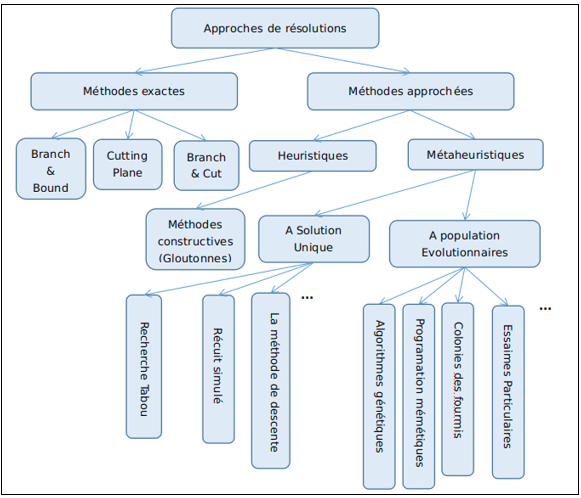
\includegraphics[width=15cm,height=6cm]{Chap3/2.png}
	\caption{Exemple de réduction du graphe G en G’}
	\label{fig:32}
\end{figure}

\end{enumerate}
	
	
Il existe deux algorithmes les plus réputé pour l construction d’un arbre  couvrant de poids minimal :  Kruskal et Prim. Nous allons se contenter de l’algorithme de Prim car d’après \cite{prim1957shortest}, c’est algorithme le plus efficace.\\


\textbf{Algorithme de Prim:}\\
C’est un algorithme  glouton qui tente à construire un arbre couvrant de poids minimal dans un graphe non orienté, connexe. Nous allons présenter dans ce qui suit l’algorithme de Prim ainsi qu’un exemple qui illustre le déroulement de ce dernier.

\begin{algorithm}[H]
\label{alg3:prim}
\caption{Prim}
\KwData{un graphe général pondéré non orienté $G=(V, E, w)$}
\KwResult{Un arbre couvrant de poids minimal T}
\SetAlgoLined
\DontPrintSemicolon

\tcp{Initialisation de T}
sommets $\gets$ un sommet de $G$ qu’on choisit \;
arêtes $\gets$ aucune 

\Repeat{tous les sommets de G soient dans T}{
Trouver toutes les arêtes de $G$ qui relient un sommet de T et un sommet extérieur à T \;
Sélectionner l’arête ayant le plus petit poids parmis l’ensemble des arêtes trouvées \;
Ajouter à T cette arête et le sommet correspondant \;
}
Retourner T \;
\end{algorithm}

\begin{figure}[H]
	\centering
	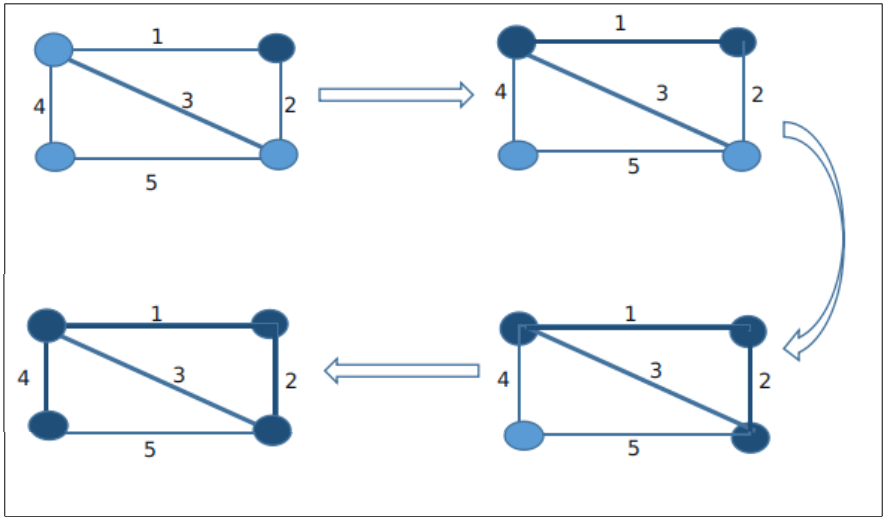
\includegraphics[width=15cm,height=8cm]{Chap3/3.png}
	\caption{illustration de l’algorithme de Prim}
	\label{fig:33}
\end{figure}


\subsection{L’élagage (Pruning):}
Cette méthode est apparue pour la première fois dans \cite{shin2010approximation,zhang2008new} et a été améliorée dans \cite{sundar2013new}.

Dans \cite{sundar2013new}, la fonction de pruning consiste à vérifié si un sommet $v \in DT$  de degré un peut être élagué  sans  que DT soit non connexe. Si cela est vérifié, ce nœud alors va devenir non dominant et l’arête incidente peut également être retirée de DT, ce qui réduit par la suite le poids de DT. Dans un second lieu, cette fonction vérifie  tous les sommets de DT dans l’ordre FIFO (First In First Out). Si le degré d’un sommet dominant v est égale à un, il est vérifié si tous les sommets adjacents à v sont également adjacents à d’autres sommets dominants dans DT. Si c’est le cas supprimer ce sommet de DT et l’arête incidente aussi. Cette méthode de pruning est largement différente que celle utilisée dans \cite{shin2010approximation} dans laquelle un arbre couvrant est d'abord construit et, par conséquent, tous les sommets feuilles peuvent être élagués sans autre vérification. 


\section{Les travaux relatifs}
Le problème de l’arbre dominant est apparu récemment (2008). Il a été introduit par \cite{zhang2008new} pour la construction d’une ossature de routage pour les réseaux sans fil avec une consommation d’énergie minimal, ce qui justifie le manque de la littérature pour ce problème. 

La consommation d’énergie est prise en compte qu’au niveau des nœuds et non les arêtes. En réalité, l'énergie consommée par chaque arête affecte directement la consommation d'énergie d'un système de routage. Par conséquent, pour minimiser la consommation d'énergie d'un système de routage, nous devons prendre en compte l'énergie consommée par chaque arête \cite{sundar2013new}.

Au meilleur de notre connaissance, aucune formulation de programmation en nombres entiers n'a été étudiée dans la littérature pour le DTP autre que celle classique introduite dans \cite{shin2010approximation}. 

En  2010, puisque le problème de l’arbre dominant est NP-hard, Yilin Shen · My T. Thai ont fait l'approximation du DTP au problème DST \cite{shin2010approximation}. Cependant, la complexité temporelle est assez élevée, du fait que la construction d'un DST entraîne généralement une longue durée d'exécution. De ce point de vue, une heuristique peu complexe en temps est souhaitable ce qui a orienté la littérature sur le DTP vers les algorithmes heuristiques, tels que la recherche par voisinage variable (VNS) et des algorithmes méta-heuristiques, tels que les algorithme génétiques, la colonie d'abeilles artificielles et les colonies de fourmis. 
Nous allons considérer pour la suite un graphe G = (V, E, w), non orienté, pondéré, où : V est l’ensemble des sommets et E est l’ensemble des arêtes du graphe G.

\subsection{L’heuristique pour le problème de l’arbre dominant (H\_DT )}
En  2013, Shyam Sundar et Alok Singh proposent un nouvel algorithme heuristique (H\_DT) pour la construction d’un arbre dominant DTP \cite{sundar2013new}. Entre autre, un arbre couvrant minimal est construit sur le sous-graphe de G induit par l’ensemble des sommets dominants de DT à l’aide de l’algorithme de Prim \cite{prim1957shortest}. De cette façon, le poids total de DT peut être réduit davantage. La raison  est que même après le pruning, le poids total de DT peut ne pas être minimum en raison de la sélection d'arêtes incorrectes lors de la construction de DT. Sur un ensemble donné de sommets dominants, de nombreux arbres dominants peuvent être construits en G. De toute évidence, un arbre dominant obtenu à l’aide de l’algorithme de Prim aura un coût minimum parmi tous ces arbres dominants. Après cela, la procédure d’élagage est à nouveau appliquée, puis un arbre couvrant minimal est à nouveau construit sur le sous-graphe de G induit par l’ensemble des sommets dominants de DT à l’aide de l’algorithme de Prim. Dans ce qui suit nous allons donner le pseudo-code de l’heuristique H\_DT et expliquer brièvement son fonctionnement:

\begin{algorithm}[H]
\label{alg3:HDT}
\caption{ pseudo-code H\_DT}
\KwData{un graphe général pondéré non orienté $G=(V, E, w)$}
\KwResult{sortie: un arbre dominant $DT \subseteq E$ }
\SetAlgoLined
\DontPrintSemicolon

\tcp{Initialise DT}
$DT \gets \varnothing $  \;

\For{chaque sommet $i \in V$}{
	Mark$[i] \gets $ 0 \;	
}

Calcule les chemins les plus courts entre toutes les paires de sommets de G \;
Triez toutes les arêtes de E en ordre non décroissant en fonction de leur poids \;

\While{tous les sommets de V ne sont pas marqués}{
Sélectionnez une arête non sélectionnée $e_{ij}$ avec un coût minimal, dont au moins un point d'extrémité n'est pas marqué \;

\For{chaque sommet v adjacent à  $i$ ou $j$ }{
	Mark$[v] \gets$ 1 \;
}

\eIf{ DT = $ \varnothing $ ou $e_{ij}$ est adjacent à une arête dans DT}{
	$ DT \gets DT \cup \{ e_{ij} \} $ \;
}{
	Trouver le chemin le plus court ST reliant DT et $\{i, j\}$ \;
	$ DT \gets DT \cup ST \cup \{ e_{ij} \}$ \;
}

\For{chaque sommet v en ST}{
	$ Mark[v] \gets 1$ \;
	\For{chaque sommet k adjacent à v }{
		$ Mark[k] \gets 1$ \;
	}
}

}

Appliquer la procédure d'élagage sur DT \;
Reconnectez les sommets dominants de DT en y construisant un arbre couvrent de poids minimal \;
Appliquer l'élagage sur le DT \; 
Reconnectez les sommets dominants de DT en y construisant un arbre couvrent de poids minimal \;
Retourner DT \;
\end{algorithm}

Cette heuristique se décompose en deux phases principales. La première phase est la phase d’initialisation, où le chemin le plus court entre toute paire de nœuds est calculé.

L’ensemble des sommets est étiqueté à "non marqué" et l’ensemble d’arêtes constituant DT est égale à l’ensemble vide. Ensuite, une phase itérative commence, où, à chaque itération, une arête eij de poids minimal avec au moins une extrémité "non marquée" est choisie. Les voisins des extrémités de l’arête ajoutée seront "marqués". Une vérification est ensuite effectuée pour déterminer si l’arête eij est adjacente à DT ou non. Si ce n’est pas le cas, alors un chemin de coût minimal est déterminé pour établir un lien entre le DT partiellement construit et l’arête sélectionnée. Les arêtes constituant ce dernier sont ajoutés à DT et les nœuds appartenant à ce chemin ainsi que leurs voisins "non-marqués" seront "marqués". Dès que tous les sommets dans V seront marqués (condition d’arrêt vérifiée ), la procédure d’élagage suivie de l’algorithme de Prim  sont appliqués.   
    
En outre, Shyam et Alok travaillent sur deux approches méta-heuristiques qui donnent des résultats satisfaisants , et ils ont essayé d’améliorer cet heuristique dans les années qui suivent.

\subsection{Colonie d'abeilles artificielle pour le DTP (ABC\_DT))}
L’algorithme de colonie d’abeilles artificielles ou Artificial Bee Colony (ABC) a été introduit par Dervis Karaboga en 2005 \cite{karaboga2005idea} et développé depuis 2005 par Karaboga et Basturk \cite{karaboga2008performance} pour les problèmes d’optimisation continue. C’est un algorithme à population, d’inspiration naturaliste, basé sur le butinage des abeilles.


\begin{enumerate}[label=\alph*)]
	
	\item \textbf{Génération de la solution initiale :}\\
	C’est un processus itératif pour générer des solutions initiales (arbres dominants) faisables, où à chaque itération, pour une probabilité P, une arête de poids minimal est choisie pour le nœud de départ qui a été choisi lui aussi aléatoirement sinon l’arête est choisie aléatoirement selon la méthode de sélection de roulette (wheel) afin de maintenir un équilibre entre qualité et diversité de la solution. A ce stade, un arbre dominant du graphe G est construit. Puis, la procédure d’élagage (décrite dans la section 3.2) est appliquée à DT de manière répétée jusqu’à ce qu’il ne soit plus possible d’élaguer un sommet dominant de degré un. Par la suite, la "procédure MST" (de la section 3.1) est appliquée sur la solution obtenue.

	\item \textbf{Probabilité de sélectionner une source alimentaire :}\\
	C’est à travers la méthode de sélection de "tournoi" dite "Binary Tournament Selection Method"(BTS), que les abeilles Onlooker (spectateurs) choisissent une solution de  la population. Avec la probabilité b t, la meilleure est choisie, sinon la pire solution est sélectionnée avec probabilité 1-bt.\\
	

\begin{algorithm}[H]
\label{alg3:ABC}
\caption{ Pseudo-code de ABC }
\SetAlgoLined
\DontPrintSemicolon

Générer $ne$ solutions aléatoires $E_1 , E_2 , ..., E_{ne}$ \;
$MeilleureSol \gets meilleure $ solution parmi $E_1 , E_2 , ..., E_{ne}$ \;

\While{La condition de terminaison est non satisfaite}{

	\For{Chaque abeille employée $i$ dans $ne$ }{
		$ E' \gets determination\_d\_ une\_solution\_voisine(E_i )$ \;
		\eIf{E' est  meilleure que $E_i$}{
			$ E_i \gets E'$ \;		
		}{
			\If{$E_i$ n'a pas changé après un nombre limité d'itérations}{
				Remplacer $E_i$ avec une solution générée aléatoirement \;
			}
		}
		\If{ $E'$ est meilleure que $MeilleureSol$}{
			$MeilleureSol \gets E_i$ \;
		}
	}
	
	\For{Chaque abeille onlooker $i$ dans $n_0$}{
		$s_i \gets méthode$ de sélection de tournoi binaire ($E_1 , E_2 , ..., E_{ne}$) \;
		$O_{ni} \gets determination\_d\_une\_solution\_voisine(E_{si})$ \;
		\If{ $O_{ni}$ est meilleure que $MeilleureSol$ }{
			$MeilleureSol \gets O_{ni} $ \;	
		}	

		\If{ $O_{ni}$ est meilleure que $E_{si}$ }{
			$E_{si} \gets O_{ni} $ \;
		}
	}
		
}

\end{algorithm}


	\item \textbf{Détermination du voisinage d’une source alimentaire:}\\
	La détermination d’une solution voisine se fait selon deux procédures qui s’excluent mutuellement. Après qu’une solution s soit crée, une copie de cette dernière est affectée à s’. Après cela, Avec une probabilité P, une solution voisine est générée en appliquant la méthode PDE, qui  supprime une arête de façon aléatoire sinon la méthode PANDV est appelée pour ajouter un sommet aléatoirement. L’application de ces deux méthodes fait que la solution devient infaisable, ce qui fait que chacune d’entre elles procède différemment pour la rendre faisable. Le pseudo-code de l’algorithme de détermination de voisinage d’ABC\_DT est représenté dans l’Algorithme \ref{alg3:PCDSV} ci-dessous.


\begin{algorithm}[H]
\label{alg3:PCDSV}
\caption{ Pseudo-code de détermination d'une solution voisine}
\KwData{Une solution s}
\KwResult{Une solution voisine s}
\SetAlgoLined
\DontPrintSemicolon

Créer une copie s' de s \;

\eIf{$u_{01} < q_1$}{
	 Appliquer la procédure PDE sur s \;
}{
	 Appliquer la procédure PANDV sur s \;
}

Appliquer la procédure pruning sur s \;
Reconnecter les sommets dominants de s’ en construisant un arbre de poids minimum sur eux (MST) \;
Appliquer la procédure pruning sur s \;
Reconnecter les sommets dominants de s’ en construisant un arbre de poids minimum sur
eux (MST) \;

\end{algorithm}

\end{enumerate}


\section{Algorithme génétique stationnaire }
C’est un algorithme génétique, dit "stationnaire" (Steady State Genetic Algorithm SSGA) \cite{sundar2014steady}, SSGA utilise la méthode de remplacement de la population à l'état d'équilibre \cite{davis1991handbook}. Cet algorithme commence par la sélection de deux parents, exécute le croisement et la mutation pour générer une solution (enfant) qui remplace le pire individu de la population. Dans ce qui suit, nous allons présenter les principales caractéristiques de cet algorithme.

\begin{enumerate}[label=\alph*)]

	\item \textbf{Génération de la solution initiale:}\\
	C’est un processus itératif, qui procède par l’ajout des arêtes de manière aléatoire dans le but d’avoir un arbre dominant. Après que cet arbre soit créé les deux procédures "pruning" de la section 3.2 et "MST" (voir la section 3.1) sont appliquées.
	
	\item \textbf{Fitness: }\\
	La Fitness d’une solution est la même que la fonction objectif d’une solution, telle que la valeur de la fonction objectif est la somme des poids des arcs de la solution.
	
	\item \textbf{La sélection:}\\
    La méthode de sélection de tournoi binaire (BTS). Cette méthode est utilisée pour la sélection d’un individu pour la mutation. Elle est utilisée aussi deux fois de façon consécutive pour la sélection de deux chromosomes (individus) comme parents pour l’opération de croisement (cross-over); avec la probabilité P, l’individu avec une meilleure fitness est sélectionné, sinon, c’est le plus mauvais qu’il l’est (avec la probabilité 1-P).
	     

	\item \textbf{Le croisement (cross-over):}\\
	Afin de générer une solution enfant C, qui est initialement vide, deux parents p1 et p2 sont sélectionnés à travers la méthode BTS.
	
Les sommets constituant la solution enfant seront choisis, en alternance, des deux ensembles des nœuds dominants des deux parents. En effet, un sommet ne sera rajouté que s’il n’existe pas déjà dans C. Maintenant, il y a une vérification sur l’existence d’une arête reliant le sommet choisi à l’arbre partiellement construit. Si c’est le cas, alors il est ajouté à C et est étiqueté à marqué ainsi que tous ses voisins. Sinon, un chemin optimal, appelé chemin potentiel, est calculé en fonction du nombre de nœuds non couverts appartenant au chemin sur le coût de celui-ci. En effet, ce chemin vise à maximiser le nombre de nœuds à rajouter dans C. De plus, cela permet d’éviter un opérateur réparateur et d’assurer d’avoir directement un arbre dominant de bonne qualité. Ce processus itératif est répété jusqu’à ce que tous les sommets soient "marqués".

	 \item \textbf{Mutation: }\\
	Cette partie commence par la sélection d’une solution initiale en utilisant la méthode BTS. Un petit ensemble $V_m$ de sommets non dominants est sélectionné aléatoirement de $V / C$.  Itérativement, un sommet $v_s \in V_m$ est de degré 1 dans G et ayant un chemin de coût minimal avec un sommet $v_c \in C$. Cette procédure se poursuit jusqu’à ce que $V_m$  devient vide. L’algorithme de Prim est ensuite appliqué à l’ensemble de sommets dominants de C.
	
	\item \textbf{Politique de remplacement:}\\
	Dans cette politique de remplacement, l’unicité de la solution enfant C, nouvellement créée, est examinée par rapport aux individus de la population. Dans le cas où C se révèle être différent de tous les individus de la population, alors il remplace le plus mauvais d’entre eux, sinon, il est rejeté.
	

\begin{algorithm}[H]
\label{alg3:PCASSGA}
\caption{ Pseudo-code de l'algorithme SSGA}
\SetAlgoLined
\DontPrintSemicolon

Générer une population (popsize) de solutions $s1 , s2 , ..., s\_pop\_size$ aléatoirement \;

$MeilleureSol \gets $ La meilleure solution de la population \;

\While{La condition de terminaison est non satisfaite}{

	\eIf{$u_{01} < p_c$}{
		$ p_1 \gets$ méthode de sélection de tournoi binaire $s1 , s2 , ..., s\_pop\_size$ \;
		$ p_2 \gets$ méthode de sélection de tournoi binaire $s1 , s2 , ..., s\_pop\_size$ \;	
		Enfant $\gets$ Opérateur de Croisement $( p1, p2 )$ \;	
	}{
		$ p_1 \gets$ méthode de sélection de tournoi binaire $s1 , s2 , ..., s\_pop\_size$ \;
		Enfant $\gets$ Opérateur de Mutation $(p1)$ \;			
	}

	\If{Enfant est un DT partiel}{
		Appliquer procédure de réparation sur Enfant \;
	} 
	
	Appliquer la procédure pruning sur le DT de Enfant \;
	Appliquer l’algorithme de Prim pour construire un arbre de poids minimal sur le sousgraphe de G induit par l’ensemble des sommets dominants de DT \;
	Appliquer la procédure pruning sur la DT de Enfant \;
	
	\If{Enfant est meilleure que $MeilleureSol$}{
		$MeilleureSol \gets Enfant$ \;  
	}
	
	Appliquer la politique de remplacement \;	
}

Retourner $MeilleureSol$ \;

\end{algorithm}


\end{enumerate}




\section{L’algorithme évolutionnaire avec mutation guidée EA/G}
L’algorithme évolutionnaire avec mutation guidée (Evolutionary algorithm with guided mutation \cite{zhang2005evolutionary} est relativement un nouveau membre de la classe des algorithmes évolutionnaires. Il a été développé par Zhang et al. (2005) \cite{zhang2005evolutionary} pour surmonter les inconvénients de deux algorithmes évolutifs, à savoir algorithmes génétiques (GAs) et estimation d'algorithmes de distribution (EDAs). Il est dit hybride car il utilise les caractéristiques des deux algorithmes cités précédemment. 

En effet, Les GAs génère une progéniture à partir des parents sélectionnés en appliquant les opérateurs génétiques tels que le croisement et la mutation. Ces algorithmes  n’utilisent que les informations de localisation des solutions et ne font pas usage des informations globales sur l’espace de recherche qui peuvent être collectées en gardant la trace de toutes les solutions générées depuis le début de l’algorithme. Dans ce contexte, "l’information de localisation d’une solution" revient à dire,l’information qui peut identifier de façon unique une solution dans l’espace de recherche de toutes les solutions. Par exemple, dans le cas du DTP, l’ensemble des arêtes formant le DT constitue son information de localisation car cette dernière peut l’identifier de façon unique.

Par ailleurs, les EDAs ne s’appuient que sur un modèle de probabilité pour générer une solution.

Le modèle de probabilité caractérise la distribution des solutions potentielles dans l’espace de recherche. Ce dernier, est mis à jour à chaque génération en utilisant des informations globales sur  l’espace de recherche extraites des individus de la génération courante. Une solution est générée en se basant sur ce modèle de probabilité. Contrairement aux GA, les EDA n'utilisent pas directement les informations de localisation des solutions \cite{chaurasia2016hybrid}. 

Pour conclure EA/G utilise un opérateur de mutation, appelé mutation guidée (GM), pour générer des descendants (solutions). La mutation guidée génère une nouvelle solution tenant compte à la fois des informations de localisation relatives à la solution mère ainsi que des informations statistiques globales relatives à l'espace de recherche. En d'autres termes, la génération d’une solution se fait par l’échantillonnage d’un modèle de probabilité caractérisant les informations statistiques globales et en copiant des éléments à partir de son parent.


\textbf{EA/G hybride pour DTP ( EA/G-MP)}\\
Cette méthode s’inspire de l’approche de Zhang et al. (2005)\cite{zhang2005evolutionary} pour le problème de la clique maximale (MCP) et est développée en 2014 par  les mêmes chercheurs. Les résultats obtenues par EA/G ont été amélioré par cette nouvelle méthode grâce à l’utilisation des deux procédures à savoir la reconnexion des nœuds de la solution via un MST (minimum spanning tree) et un opérateur d’élagage. Néanmoins, chacune de ces procédures est appliquée deux fois dans l'ordre MST $\to$ Pruning $\to$ MST $\to$ Pruning.

Pour commencer EA/G-MP, nous devant définir les voisins de chaque nœud $v \in V$ et de calculer le chemin le plus court entre toute paire de nœuds. Avant de passer aux caractéristiques de l’algorithme, nous présentons dans ce qui suit un pseudo-code pour la procédure << pruning >>  pour cette approche suivit d’une explication pour ce dernier :\\

\begin{algorithm}[H]
\label{alg3:PCPP}
\caption{Pseudo-code de la procédure pruning}
\SetAlgoLined
\DontPrintSemicolon

$R_n \gets  \{ v : v \in DN$ et $|ON ( v ) \cap DN | = 1$ et $CN(v) \subseteq (\cup_{u \in DN  \setminus \{  v  \} } ) \} $ \;

\While{ $R_n \neq \varnothing$ }{

	$DN \gets DN \setminus \{ v \}$ \;
	$R_n \gets  \{ v : v \in DN$ et $|ON ( v ) \cap DN | = 1$ et $CN(v) \subseteq (\cup_{u \in DN  \setminus \{  v  \} } ) \} $ \;	
}

Retourner DN \;

\end{algorithm}

Puisque le rôle de la procédure d’élagage consiste à éliminer les nœuds redondants dans l’arbre dominant. Pour cela, Cette procédure commence tout d’abord à sélectionner tous ces  nœuds où le degré de chaque nœud v dans DN est égal à un et tous les nœuds voisins non dominants du nœud v sont couverts par d'autres nœuds dominants (autres que le nœud v) dans DN. Puis, un processus itératif commence: lors de chaque itération, un nœud de l’ensemble Rn est sélectionné ( la sélection se fait selon l’ordre FIFO) et est supprimé de DN ainsi que de Rn. 

De plus, tout en construisant un arbre dominant, la convention suivie, est celle où : un nœud prend la couleur BLANCHE s’il n’est pas un nœud dominant et n’est pas adjacent à un nœud dominant, GRISE si ce nœud est adjacent à un nœud dominant mais il ne l’est pas ,et un nœud appartenant à l’arbre est supposé avoir la couleur NOIRE. Initialement, tous les nœuds sont supposés avoir la couleur BLANCHE. Lorsque la construction de l’arbre dominant est terminée, les nœuds appartenant à l’arbre auront la couleur NOIRE et tous les autres nœuds (non dominants) auront la couleur GRISE.

\begin{enumerate}[label=\alph*)]
	
	\item \textbf{Solution initiale:}\\
	Avant de présenter cette méthode commençons à définir quelques variables utilisées: 
$W_n$ : ensemble de nœuds BLANCs ($W_n$ = V Initialement).
$I_u$ : l’ensemble des nœuds non dominants.
$n_b$ : Ensemble de nœuds BLANCs voisins à v i.e. : $nb = ON(v) \cup W_n$.
La méthode de génération de solution initiale est la même que celle utilisée dans Sundar et Singh (2013)(ABC\_DT) \cite{sundar2013new} en portant deux modifications : La première, est que seuls les arrêtes $e_{vu}$ sont considérés où $u \in I_u$ a au moins un voisin BLANC, c’est-à-dire où | ON(u) $W_n$ | $\geq$ 1. La deuxième modification, est qu'avec la probabilité $1 - \phi $, nous sélectionnons les arrêtes uniformément au hasard au lieu d’utiliser la méthode de sélection de ABC\_DT.

\begin{algorithm}[H]
\label{alg3:PCSIEAGMP}
\caption{Pseudo-code de la solution initiale de EA/G-MP}
\SetAlgoLined
\DontPrintSemicolon

Initialement tous les nœuds dans V sont colorés en BLANC \;
$W n \gets V \, DT \gets \varnothing \, DN \gets \varnothing \, I_u \gets \varnothing $ \;

$v \gets Random(W_n)$ \;
$ DN \gets DN \cup \{ v \} $ \;
Mettre v NOIR \;
$ nb \gets ON( v ) \cap W_n $ \;
$ W_n \gets W_n \setminus ( nb \cup \{ v \})$ \;

Mettre tous les noeuds $\in$ nb GRIS \;
$I_u \gets nb$ \;

\While{ $W_n \neq \varnothing$}{
	Générer un nombre aléatoire $u_{01}$ tel que $0 \leq u_{01} \leq 1$ \;
	\eIf{$u_{01} < \phi $}{
		$(v,u) \gets $ argument $ v \in DN, \{ u \in I_u |ON(u) \cap W_n| \, \geq 1 \} w(v,u)$ \;
	}{
		$ v \gets Random(DN)$ \;			
		$ u \gets \{ u:Random(I_u)$ et $|ON(u) \cap W_n| \, \geq 1 \} $
	}
	$DT \gets DT \cup \{ e_{v,u}  \} $	\;
	$DN \gets DN \cup \{ u \} $	\;
	Mettre u NOIR \;
	$I_u \gets I_u \setminus \{ u \} $ \;
	$ nb \gets \{ u: u \in ON(u) \cap W_n \} $ \;
	Mettre tous les noeuds nb GRIS \;
	$I_u \gets I_u \cup nb $	\;
	$W_n \gets W_n \setminus nb$ \;	
}

Appliquer la procédure pruning sur les nœuds dans DT \;
Reconnecter les nœuds dans DT via MST \;
Retourner DT \;

\end{algorithm}


	\item \textbf{Initialisation et mise à jour du vecteur de probabilités}\\
	Le vecteur de probabilité est définit comme suit: p = {p1, p2, ..., p|V|} [0, 1]$^{|V|}$, où | V | est le nombre de nœuds dans l'ensemble V (nombre de nœuds dans le graphe G), p est la probabilité que le nœud $v \in V$ soit présent dans un arbre dominant. Ce vecteur est initialisé  avec le rapport entre le nombre de solutions initiales contenant ce nœud et le nombre total de solutions initiales. Le pseudo-code est présenté dans l'algorithme \ref{alg3:IVPEAMP}.
	
\begin{algorithm}[H]
\label{alg3:IVPEAMP}
\caption{Pseudo-code de l'initialisation du vecteur de probabilités de EA/G-MP.}
\SetAlgoLined
\DontPrintSemicolon

$ nv \gets $ nombre de solutions initiales contenant le nœud $v, \forall v \in V$ ;

$ pv \gets$ \( \displaystyle \frac{nv}{Np} \) ,  $\forall v \in V $ \;


\end{algorithm}

A chaque génération g, un ensemble parent "parent (g)" est formé en sélectionnant les meilleures solutions L dans la population actuelle (g). Une fois que le parent (g) est formé, il est utilisé pour mettre à jour le vecteur de probabilité p. Le pseudo-code pour la mise à jour du vecteur de probabilité est donné dans l’algorithme \ref{alg3:MAJVPEAMP}.

\begin{algorithm}[H]
\label{alg3:MAJVPEAMP}
\caption{Pseudo-code de la mise à jour du vecteur de probabilités de EA/G-MP.}
\SetAlgoLined
\DontPrintSemicolon

$ nv \gets $ nombre de solutions initiales contenant le nœud $v, \forall v \in V$ ;

$ pv \gets ( 1 - \lambda ) pv + \lambda \,$ \( \displaystyle \frac{nv}{L} \)  $\, \, , \forall v \in V $ \;

\end{algorithm}	
	
	
où: $\lambda \in [ 0, 1 ] $  est le taux d’apprentissage ; plus $\lambda$ est grand, plus la contribution des solutions dans parent (g) est grande.
nv: Le nombre total de solution contenant dans le parent (g).

	
	\item \textbf{Opérateur de mutation guidée GM}\\
	L'opérateur GM utilise à la fois les informations statistiques globales stockées sous la forme du vecteur de probabilité p et les informations de localisation de la solution parent pour générer de nouveaux individus. Le pseudo-code de l'opérateur GM est présenté dans l'algorithme \ref{alg3:PCGM}.
	
où $\beta \in [0, 1]$ est un paramètre ajustable et DT est un nouvel arbre dominant construit par l'opérateur GM et dont les nœuds sont soit choisi aléatoirement selon le vecteur de probabilité p, soit ils sont copiés à partir  de la solution mi de la population courante. 

Le choix des nœuds à partir de mi peut aider à améliorer la qualité de la solution vu que celle-ci fait parti des meilleures solutions M, cependant, l’utilisation du vecteur de probabilités permet une meilleure diversification en ajoutant les nœuds les moins utilisés a travers les générations.
	
	
\begin{algorithm}[H]
\label{alg3:PCGM}
\caption{Pseudo-code de GM}
\SetAlgoLined
\DontPrintSemicolon

Mettre la couleur de tous les nœuds dans V à BLANC \;
$ DT \gets \varnothing $ \;
\For{nœud $v \in V$ dans un ordre quelconque}{
	Générer un nombre aléatoire $r_1$ tel que $ 0 \leq r_1 \leq 1 $ \;
	\eIf{$ r_1 < \beta $}{
		Générer un nombre aléatoire $r_2$ tel que $ 0 \leq r_2 \leq 1 $ \;
		\If{ $r_2 < p v $ Et ((v est BLANC) Ou (v est GRIS avec au moins un voisin BLANC))}{
		   Trouver le chemin le plus court SP entre le nœud v et un nœud u dans DT\;
		   Ajouter toutes les arêtes de SP dans DT \;
		   Colorer en NOIR tous les nœuds dans le chemin SP \;
		   Colorer en GRIS tous les nœuds voisins BLANCs des nœuds sur le chemin SP\;
		}
	}{
		\If{v est un nœud dominant dans m i et v est GRIS avec au moins un voisin 					BLANC}
		{
		   Trouver le chemin le plus court SP entre le nœud v et un nœud u dans DT\;
		   Ajouter toutes les arêtes de SP dans DT \;
		   Colorer en NOIR tous les nœuds dans le chemin SP \;
		   Colorer en GRIS tous les nœuds voisins BLANCs des nœuds sur le chemin SP\;
		}
	}
}

Retourner DT \;

\end{algorithm}


L’opérateur de mutation GM ne garanti pas la faisabilité de la. Pour cette raison,  toutes les solutions infaisables générées par cet opérateur sont traitées par un opérateur de réparation de façon à ce qu’elles deviennent réalisables.


\item \textbf{Opérateur de réparation:}
L’opérateur de réparation s’applique uniquement sur une solution infaisable générée par l’opérateur GM. Car de l'application de ce dernier, peut résulter des nœuds non couvrants. Pour résoudre ce problème,  l’opérateur de correction procède comme suit:
  
soit $U_{cn}$ l’ensemble des nœuds non couvrants (blancs) restants. Tous d’abord, un nœud contenant le nombre  le plus élevé de nœuds voisins blancs dans la liste $U_{cn}$ est sélectionné. Si aucun des nœuds de l’ensemble $U_{cn}$ n’a des nœuds voisins BLANCS, le nœud ayant l’indice le plus bas est sélectionné à partir de $U_{cn}$ , ce nœud est nommé i. Après cela, le chemin le plus court entre le nœud i et l’arbre partiellement construit DT est calculé, et toutes les arêtes de ce dernier sont ajoutées dans DT. De même, les nœuds de ce chemin sont recolorés en NOIR (si ce n’est pas déjà fait) et leurs nœuds voisins en GRIS. Tous ces nœuds NOIR et GRIS sont ensuite supprimés de l’ensemble $U_{cn}$ . Ce processus itératif  est répété jusqu’à ce que $U_{cn}$ devient vide. Le pseudo-code de l’opérateur de réparation est donné dans l’Algorithme \ref{alg3:PCOR} suivant:

\begin{algorithm}[H]
\label{alg3:PCOR}
\caption{Pseudo-code de l’opérateur de réparation}
\SetAlgoLined
\DontPrintSemicolon

\While{ $U_{cn} = \varnothing$ }{
	$v \gets - argmax \, u \in U_{cn} (wd(u) > 0) $ \;
	\If{  $ v \neq \varnothing $ }{
		Sélectionner un nœud v avec le plus petit index de $U_{cn}$ ;
	}	
	
	Trouver le chemin le plus court SP entre le nœud v et un nœud u dans DT \;
	Ajouter toutes les arêtes de SP dans DT \;
	Colorer en NOIR tous les nœuds dans le chemin SP \;
	Colorer en GRIS tous les nœuds voisins BLANCs des nœuds sur le chemin SP \;
	Enlever tous les nœuds NOIRs et GRIS de $U_{cn}$ \;
}

Retourner DT \;

\end{algorithm}


Le pseudo-code de l’approche EA/G-MP pour DTP est donné dans l'algorithme \ref{alg3:EAMPDTP}.

\begin{algorithm}[H]
\label{alg3:EAMPDTP}
\caption{EA/G-MP pour DTP}
\SetAlgoLined
\DontPrintSemicolon

A la génération $g \gets 0 $ , une population initiale pop(g) qui consiste en N p solutions est générée aléatoirement \;

Initialiser le vecteur de probabilités p pour tous les nœuds en utilisant l’Algorithme \ref{alg3:IVPEAMP} \;

\While{La condition de terminaison est non satisfaite}{\;

	Sélectionner les L meilleures solutions de pop(g) pour former un ensemble parent
	parent(g), puis mettre à jour le vecteur de probabilités p en utilisant 				l’Algorithme \ref{alg3:MAJVPEAMP} \;\;

	Appliquer l’opérateur de mutation guidée GM une fois sur chacune des M meilleures
	solutions. Un opérateur de réparation est appliqué sur chaque solution générée, 		si nécessaire, puis MST, l’opérateur de pruning, MST et l’opérateur de pruning 			sont appliqués sur chaque solution générée pour améliorer sa fitness. Ajouter 			toutes les M nouvelles solutions générées avec N p - M meilleures solutions à 			pop(g) pour former pop(g+1). Si le critère d’arrêt est satisfait, retourner 			l’arbre dominant avec le poids minimum trouvé jusqu’à présent \;\;

	$ g \gets g + 1 $ \;

	\If{la meilleure solution de la population ne s’améliore pas après S générations}		{
		réinitialiser toute pop(g), sauf la meilleure solution, puis initialiser le 			vecteur de probabilités p pour tous les nœuds en utilisant l’Algorithme 				\ref{alg3:IVPEAMP}	
	}
	
}

\end{algorithm}


\end{enumerate}


\section{Conclusion}
Dans ce chapitre nous avons présenté le problème de l’arbre dominant, qui est une des approches utilisées pour la résolution du problème de consommation de l’énergie dans les réseaux de capteurs sans fil. Comme la construction de DT est NP-hard, Shin et Thai ont proposé une approximation de ce dernier en DST pour optimiser le temps de construction de l’arbre dominant \cite{shin2010approximation}, et d’autre chercheurs ont opté pour le développement des méta-heuristiques pour la même raison. Cependant, on ne peut pas tout avoir dans une méta-heuristique (c’est à dire qu’une méta-heuristique peut donner des meilleurs résultats en terme temps de calcul et d’autre en terme de qualité de solution) pourquoi ne pas penser à combiner des méta-heuristiques pour des résultats plus fiables?.

 